\documentclass{article}
\usepackage[utf8]{inputenc}
\usepackage{listings}
\usepackage[a4paper, total={6in, 9in}]{geometry}
\title{Deep Learning and Artificial Neural Networks \\ Homework 3 \\ Convolutional Neural Network}
\author{Author: Ramin Mammadzada \\ Student no: 16568003}
\date{27 December 2017}

\usepackage{natbib}
\usepackage{graphicx}

\begin{document}

\maketitle

\tableofcontents  

\newpage

\section{Convolution Neural Network}
\subsection{Introduction}
Convolutional Neural Networks are very similar to ordinary Neural Networks. They are made up of neurons that have learnable weights and biases. Each neuron receives some inputs, performs a dot product and optionally follows it with a non-linearity. The whole network still expresses a single differentiable score function: from the raw image pixels on one end to class scores at the other. And they still have a loss function (e.g. SVM/Softmax) on the last (fully-connected) layer and all the tips/tricks that is developed for learning regular Neural Networks still apply. \\
ConvNet architectures make the explicit assumption that the inputs are images, which allows us to encode certain properties into the architecture. These then make the forward function more efficient to implement and vastly reduce the amount of parameters in the network.

\subsection{General view of CNN}
Convolutional Neural Networks take advantage of the fact that the input consists of images and they constrain the architecture in a more sensible way. In particular, unlike a regular Neural Network, the layers of a ConvNet have neurons arranged in 3 dimensions: width, height, depth. For example, the input images in CIFAR-10 are an input volume of activations, and the volume has dimensions 32x32x3 (width, height, depth respectively). The neurons in a layer will only be connected to a small region of the layer before it, instead of all of the neurons in a fully-connected manner. Moreover, the final output layer would for CIFAR-10 have dimensions 1x1x10, because by the end of the ConvNet architecture we will reduce the full image into a single vector of class scores, arranged along the depth dimension. The visualization of this is below:

\begin{figure}[h!]
	\centering
	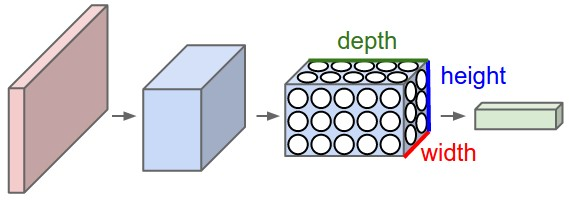
\includegraphics[scale=0.55]{model1.jpeg}
	\caption{CNN Model overview}
	\label{fig:univerise}
\end{figure}

\section{Application of CNN}

\subsection{Hand Sign Detection System}
I found a hand sign dataset that is a collection of 6 signs representing numbers from 0 to 5 (as shown in the picture below). Using TensorFlow framework for Convolutional Neural Network I created a model to recognize hand sign and trained it for 20 epoch.

\begin{figure}[h!]
	\centering
	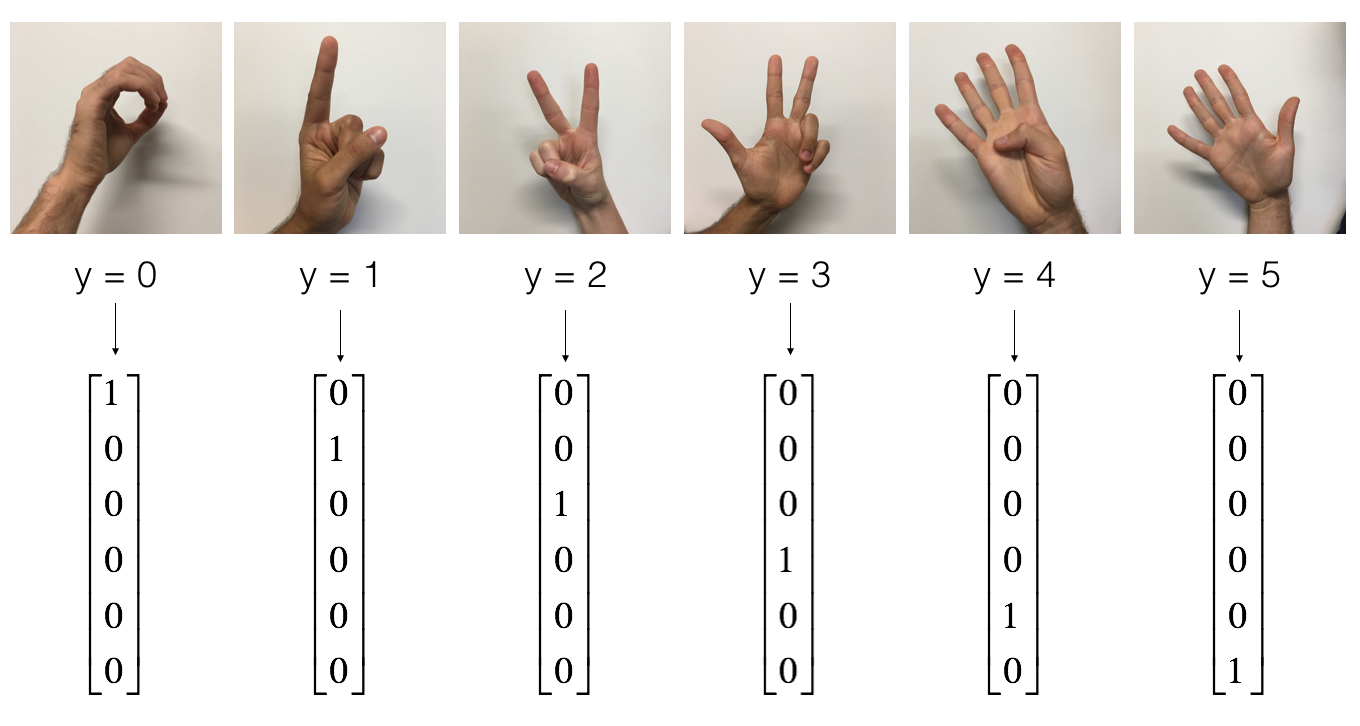
\includegraphics[scale=0.55]{SIGNS.png}
	\caption{CNN Model overview}
	\label{fig:univerise}
\end{figure}

\newpage

TensorFlow requires that we create placeholders for the input data that will be fed into the model when running the session. Then, before the forward propagation,I initialized weights/filters  W1  and  W2. Tensorflow arranges bias variables automatically, there is no need to add it.

In the forward propagation, I followed this style to create a model:
\begin{figure}[h!]
	\centering
	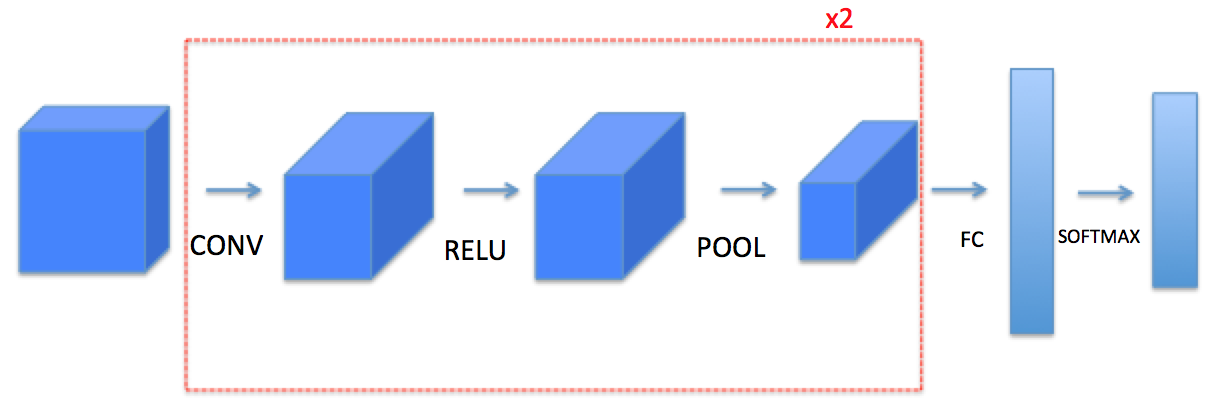
\includegraphics[scale=0.55]{model.png}
	\caption{CNN Model overview}
	\label{fig:univerise}
\end{figure}


In detail, I used the following parameters for all the steps:

\begin{itemize}
	\item Conv2D: stride 1, padding is "SAME"\
	\item ReLU
	\item Max pool: Use an 8 by 8 filter size and an 8 by 8 stride, padding is "SAME"
	\item Conv2D: stride 1, padding is "SAME"
	\item ReLU
	\item Max pool: Use a 4 by 4 filter size and a 4 by 4 stride, padding is "SAME"
	\item Flatten the previous output.
	\item FULLYCONNECTED (FC) layer: Apply a fully connected layer without an non-linear activation function.
\end{itemize}

\subsection{Results}
Firstly, I choosed learning rate of 0.009. After 100 epoch, the cost still going down as it is shown in the Figure 4 below. So it means it worth to run it a little bit more.

\begin{figure}[h!]
	\centering
	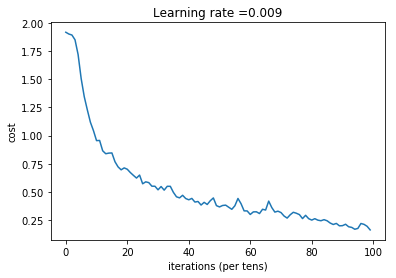
\includegraphics[scale=0.55]{result009ep100.png}
	\caption{Cost vs epoch (Train Accuracy: 0.940741 ,  Test Accuracy: 0.783333)}
	\label{fig:univerise}
\end{figure}

Therefore, I let it try 140 epoch with 0.009 learning rate to find the optimal  stopping point for epoch. As depicted in Figure 5, test accuracy stayed same and the train accuracy has a small fluctuation. So, the optimal epoch , when the learning rate is 0.009, can be selected around 110.
\begin{figure}[h!]
	\centering
	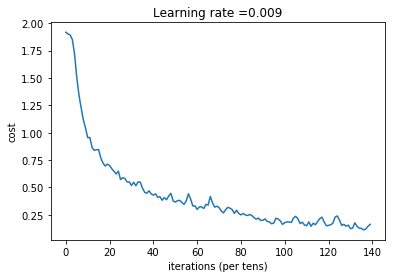
\includegraphics[scale=0.55]{result009ep140.png}
	\caption{Cost vs epoch (Train Accuracy: 0.948148 ,  Test Accuracy: 0.783333)}
	\label{fig:univerise}
\end{figure}

When I changed learning rate to 0.09 instead of 0.009 with the 100 epoch, the cost rapidly decresed to around 1.90 as shown in the Figure 6, but the train and test accuracy were not got at all, about 0.166 for both.

\begin{figure}[h!]
	\centering
	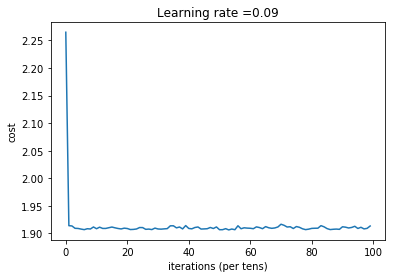
\includegraphics[scale=0.55]{result09ep100.png}
	\caption{Cost vs epoch (Train Accuracy: 0.166667,  Test Accuracy: 0.166667)}
	\label{fig:univerise}
\end{figure}

\newpage

Instead of increasing, by decreasing the learning rate to 0.0045, I run the model for 140 epoch. As shown in the Figure 7, the cost became around 0.045 after 130 epoch. The test and train accuracies also the best results I get till now.

\begin{figure}[h!]
	\centering
	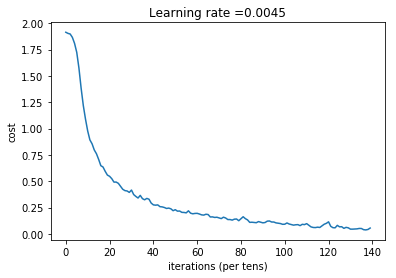
\includegraphics[scale=0.55]{result0045ep140.png}
	\caption{Cost vs epoch (Train Accuracy: 0.997222,  Test Accuracy: 0.866667)}
	\label{fig:univerise}
\end{figure}

Lastly, by decreasing learning rate to 0.0025, again I run the model for 140 epoch. The train accuracy decreased a little bit, but there is a small rise in the test accuracy. The cost is continue to decrease in the Figure 8, so it worth to increase the epoch to find the best point to stop. The increases till 0.11 . In the Figure 9, We can see that the optimal epoch time is around 150. Because the train accuracy is 0.9787 and the test accuracy is the best one till now.

\begin{figure}[h!]
	\centering
	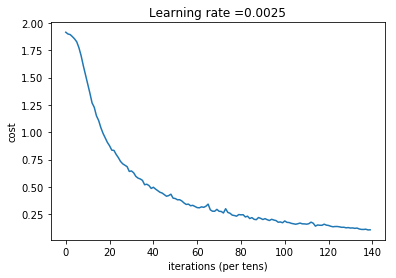
\includegraphics[scale=0.55]{result0025ep140.png}
	\caption{Cost vs epoch (Train Accuracy: 0.974074,  Test Accuracy: 0.875)}
	\label{fig:univerise}
\end{figure}

\begin{figure}[h!]
	\centering
	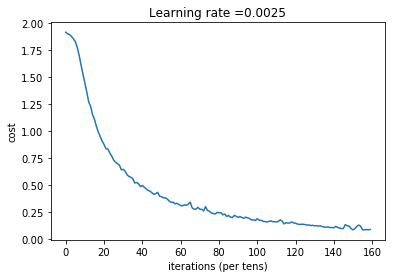
\includegraphics[scale=0.55]{result0025ep160.png}
	\caption{Cost vs epoch (Train Accuracy: 0.978704,  Test Accuracy: 0.891667)}
	\label{fig:univerise}
\end{figure}


\newpage
\bibliographystyle{plain}

\end{document}







%-----------------------------------
\begin{lstlisting}
import numpy as np

def incmatrix(genl1,genl2):
m = len(genl1)
n = len(genl2)
M = None #to become the incidence matrix
VT = np.zeros((n*m,1), int)  #dummy variable

#compute the bitwise xor matrix
M1 = bitxormatrix(genl1)
M2 = np.triu(bitxormatrix(genl2),1) 

for i in range(m-1):
for j in range(i+1, m):
[r,c] = np.where(M2 == M1[i,j])
for k in range(len(r)):
VT[(i)*n + r[k]] = 1;
VT[(i)*n + c[k]] = 1;
VT[(j)*n + r[k]] = 1;
VT[(j)*n + c[k]] = 1;

if M is None:
M = np.copy(VT)
else:
M = np.concatenate((M, VT), 1)

VT = np.zeros((n*m,1), int)

return M
\end{lstlisting}

\lstinputlisting[language=Python, firstline=3, lastline=7]{Hello.py}